\documentclass[10pt,aspectratio=169]{beamer}

% Theme and color setup
\usetheme{Boadilla}
\usecolortheme{dolphin}

% Custom colors
\definecolor{primarygreen}{HTML}{2E7D32}
\definecolor{lightgreen}{HTML}{558B2F}
\definecolor{darkgreen}{HTML}{1B5E20}

% Color customization
\setbeamercolor{frametitle}{fg=primarygreen}
\setbeamercolor{title}{fg=primarygreen}
\setbeamercolor{structure}{fg=primarygreen}
\setbeamercolor{item}{fg=darkgreen}
\setbeamercolor{block title}{bg=lightgreen,fg=white}
\setbeamercolor{block body}{bg=lightgreen!20}

% Packages
\usepackage[utf8]{inputenc}
\usepackage[spanish,english]{babel}
\usepackage{graphicx}
\usepackage{booktabs}
\usepackage{array}

% Custom commands
\newcommand{\emoji}[1]{\raisebox{-0.1ex}{\includegraphics[height=0.8em]{../emojis/#1}}}
\newcommand{\here}{\textbf{\textcolor{red}{\Huge HASTA ACÁ LLEGUE!}}}
\newcommand{\wtf}[1]{"\textbf{#1} \emoji{wtf}"}

% Title page information
\title{\emoji{wtf} XAI: Understanding Course Foundations and Motivations}
\author{FAMAF - UNC}
\date{\today}
\titlegraphic{\includegraphics[width=4cm]{../../assets/logo.jpeg}}

\begin{document}

% Title frame
\begin{frame}
\titlepage
\end{frame}

% Disclaimer
\begin{frame}{Disclaimer}
\begin{block}{This course is based on}
\textbf{Explainable Artificial Intelligence}

From Simple Predictors to Complex Generative Models\\
Spring 2023, Harvard University

\url{https://interpretable-ml-class.github.io/}
\end{block}
\end{frame}

% Agenda
\begin{frame}{Agenda}
\begin{itemize}
\item Course Goals \& Logistics
\item Model Understanding: Use Cases
\item Inherently Interpretable Models vs. Post-hoc Explanations
\item Defining and Understanding Interpretability
\end{itemize}
\end{frame}

% Goals of this Course
\begin{frame}{Goals of this Course}
Learn and improve upon the state-of-the-art literature on ML interpretability and explainability:

\begin{itemize}
\item Understand where, when, and why is interpretability/explainability needed
\item Read, present, and discuss research papers
\item Formulate, optimize, and evaluate algorithms
\item Implement state-of-the-art algorithms; Do research!
\item Understand, critique, and redefine literature
\end{itemize}

\vspace{0.5cm}
\centering
\textbf{\Large EMERGING FIELD!!}
\end{frame}

% Course Overview
\begin{frame}{Course Overview}
\begin{enumerate}
\item \textbf{Foundations and Human Factors} - definitions, taxonomies, and cognitive aspects
\item \textbf{Interpretability and Explainability Methods} - inherently interpretable models and post-hoc explanations
\item \textbf{Advanced Techniques and Evaluation} - attention-based explanations and quality metrics
\item \textbf{Interpretability of Large Models} - mechanistic interpretability and LLM understanding
\item \textbf{Emerging Frontiers of XAI} - automated circuit discovery and multimodal techniques
\end{enumerate}
\end{frame}

% Who should take this course?
\begin{frame}{Who should take this course?}
\begin{itemize}
\item Course particularly tailored to students interested in \textbf{research} \emoji{test-tube} on interpretability/explainability
\begin{itemize}
\item \textbf{Not a surface level course! \emoji{fire}}
\item \textbf{Not just applications! \emoji{fire}}
\end{itemize}
\item Goal is to push you to question existing work and make new contributions to the field
\end{itemize}
\end{frame}

% Class Format
\begin{frame}{Class Format}
\begin{itemize}
\item Course comprises of lectures, guests, and student presentations
\item Each lecture will cover: at least 2 papers \emoji{page-facing-up} \emoji{page-facing-up}
\item Students are \textbf{expected} to "at least" skim through the papers beforehand \emoji{yawning-face}
\item Students will divide into groups
\end{itemize}

\vspace{0.5cm}
\textbf{Each breakout group is expected to come up with:}
\begin{itemize}
\item A list of 2 to 3 weaknesses of each of the works discussed
\item Strategies for addressing those weaknesses
\end{itemize}
\end{frame}

% Course Components
\begin{frame}{Course Components}
\textbf{Research project (60\%)}
\begin{itemize}
\item 3 checkpoints (10\% each) – Proposal + Baseline Implementation + Midterm Progress
\item Final Report (20\%)
\item Final Presentation (10\%)
\item Teams of 2 to 3
\end{itemize}

\textbf{Research Paper Presentation (30\%)}
\begin{itemize}
\item Teams of 2; Each team presents two papers in the class
\end{itemize}

\textbf{Class Participation (10\%)}
\begin{itemize}
\item Being active in discussions in class
\item Attending classes
\end{itemize}
\end{frame}

% Research Projects
\begin{frame}{Research Projects - AKA Final Exam}
\begin{block}{Requirements}
\begin{itemize}
\item Short research paper (max 4 pages)
\item Teams of 2 students
\item Target: Local conference submission
\end{itemize}
\end{block}

\begin{block}{Assessment}
\begin{itemize}
\item Ongoing feedback from entire course
\item Course approved when paper is submitted
\end{itemize}
\end{block}
\end{frame}

% Background
\begin{frame}{Background}
\textbf{Understanding:}
\begin{itemize}
\item Linear algebra
\item Probability
\item Algorithms
\item Machine learning
\item Programming in Python, Numpy, Sklearn
\end{itemize}

\textbf{Familiarity with:}
\begin{itemize}
\item Statistics
\item Optimization
\end{itemize}
\end{frame}

% Motivation
\begin{frame}{Motivation}
\begin{block}{Machine Learning is EVERYWHERE!! \cite{lipton2016mythos}}
\centering
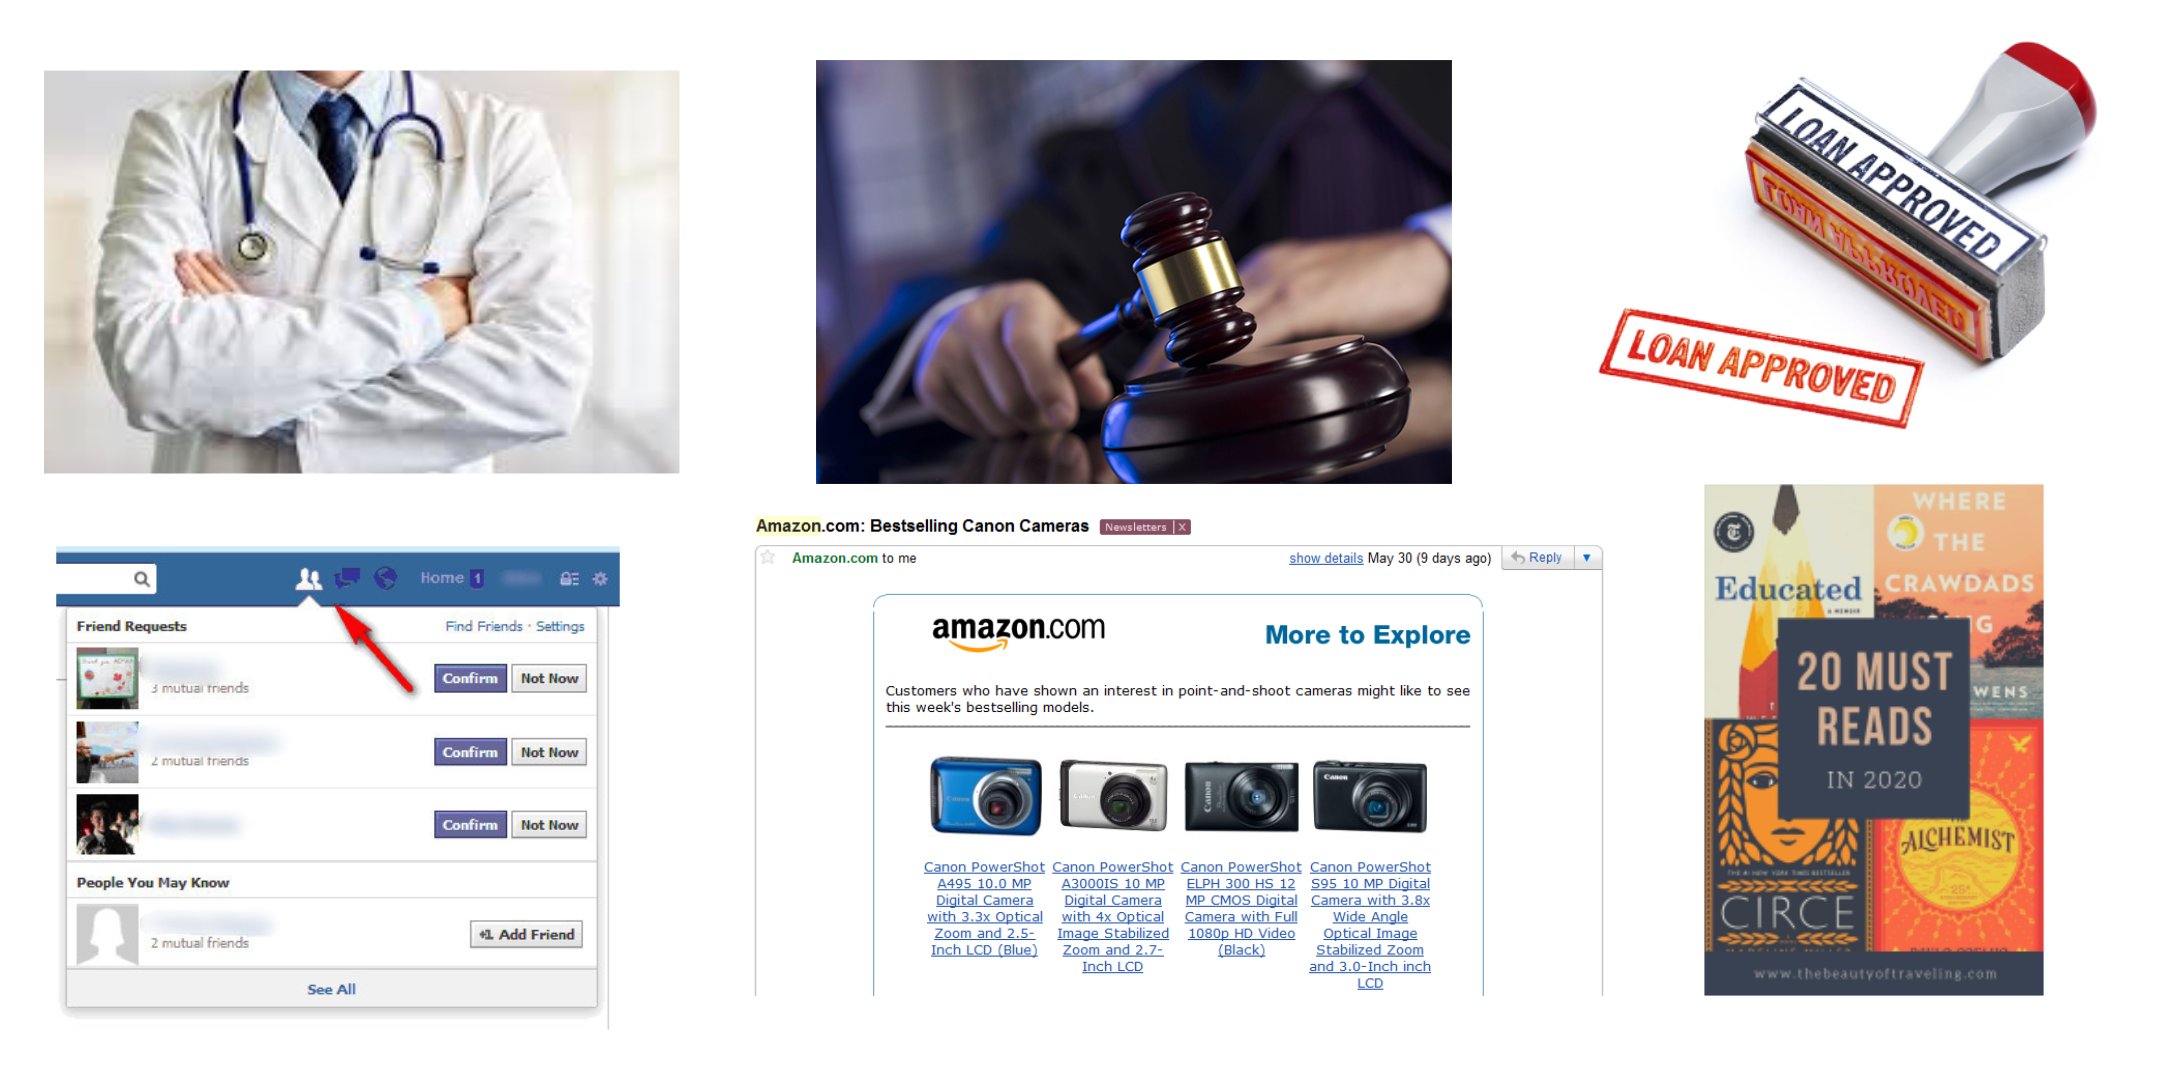
\includegraphics[width=4cm]{imgs/motivation.png}
\end{block}
\end{frame}

% Model understanding facilitates debugging
\begin{frame}{Motivation: Why Model Understanding?}
\begin{block}{Model understanding facilitates debugging}
\textbf{Example:} Image classification model
\begin{itemize}
\item Input: Dog in snow
\item Prediction: Siberian Husky
\item \textbf{Problem:} Model relies on snow background, not dog features
\item \textbf{Solution:} Model understanding reveals incorrect feature usage
\end{itemize}
\end{block}
\end{frame}

% Model understanding facilitates bias detection
\begin{frame}{Motivation: Why Model Understanding?}
\begin{block}{Model understanding facilitates bias detection}
\textbf{Example:} Criminal justice risk assessment
\begin{itemize}
\item Input: Defendant details
\item Prediction: High risk to release
\item \textbf{Problem:} Model uses race and gender inappropriately
\item \textbf{Solution:} Model understanding reveals biased features
\end{itemize}

\vspace{0.3cm}
\textit{[Larson et. al. 2016]}
\end{block}
\end{frame}

% Model understanding helps provide recourse
\begin{frame}{Motivation: Why Model Understanding?}
\begin{block}{Model understanding helps provide recourse}
\textbf{Example:} Loan application system
\begin{itemize}
\item Input: Applicant financial data
\item Prediction: Loan denied
\item \textbf{Solution:} Model explains actionable steps:
\begin{itemize}
\item "Increase salary by \$50K"
\item "Pay credit card bills on time for next 3 months"
\end{itemize}
\end{itemize}
\end{block}
\end{frame}

% Model understanding helps assess when to trust predictions
\begin{frame}{Motivation: Why Model Understanding?}
\begin{block}{Model understanding helps assess when to trust predictions}
\textbf{Example:} Medical diagnosis system
\begin{itemize}
\item Different logic for male vs. female patients
\item For females: Uses irrelevant ID number
\item For males: Uses relevant symptoms
\item \textbf{Decision:} Don't trust predictions for female subpopulation
\end{itemize}
\end{block}
\end{frame}

% Summary of Use Cases
\begin{frame}{Motivation: Why Model Understanding?}
\begin{block}{Summary of Use Cases}
\begin{table}
\centering
\begin{tabular}{ll}
\toprule
\textbf{Utility} & \textbf{Stakeholders} \\
\midrule
Debugging & Researchers and engineers \\
Bias Detection & Regulatory agencies (FDA, European commission) \\
Recourse & End users (loan applicants) \\
Trust Assessment & Decision makers (doctors, judges) \\
Deployment Vetting & Regulatory agencies \\
\bottomrule
\end{tabular}
\end{table}
\end{block}
\end{frame}

% Take 1: Build inherently interpretable predictive models
\begin{frame}{Achieving Model Understanding}
\begin{block}{Take 1: Build inherently interpretable predictive models}
Examples:
\begin{itemize}
\item Linear regression
\item Decision trees
\item Rule-based models
\end{itemize}

\vspace{0.3cm}
\textit{[Letham and Rudin 2015; Lakkaraju et. al. 2016]}
\end{block}
\end{frame}

% Take 2: Explain pre-built models in a post-hoc manner
\begin{frame}{Achieving Model Understanding}
\begin{block}{Take 2: Explain pre-built models in a post-hoc manner}
\centering
Black Box Model → \textbf{Explainer} → Human-interpretable explanation

\vspace{0.5cm}
\textit{[Ribeiro et. al. 2016, 2018; Lakkaraju et. al. 2019]}
\end{block}
\end{frame}

% Accuracy-Interpretability Trade-offs
\begin{frame}{Inherently Interpretable Models vs. Post hoc Explanations}
\begin{block}{Accuracy-Interpretability Trade-offs}
In certain settings, accuracy-interpretability trade offs may exist.

\textbf{Example scenarios:}
\begin{itemize}
\item Simple boundary: Can build interpretable + accurate models
\item Complex boundary: Complex models might achieve higher accuracy
\end{itemize}

\vspace{0.3cm}
\textit{[Cireşan et. al. 2012, Caruana et. al. 2006, Frosst et. al. 2017, Stewart 2020]}
\end{block}
\end{frame}

% Sometimes, you don't have enough data
\begin{frame}{Inherently Interpretable Models vs. Post hoc Explanations}
\centering
\textbf{Sometimes, you don't have enough data to build your model from scratch.}

\vspace{0.5cm}
\textbf{And, all you have is a (proprietary) black box!}

\vspace{0.5cm}
\textit{[Ribeiro et. al. 2016]}
\end{frame}

% Recommendation
\begin{frame}{Inherently Interpretable Models vs. Post hoc Explanations}
\begin{block}{Recommendation}
\textbf{If you can build an interpretable model which is also adequately accurate for your setting, DO IT!}

\vspace{0.5cm}
\textbf{Otherwise, post hoc explanations come to the rescue!}
\end{block}
\end{frame}

% Motivation for Interpretability
\begin{frame}{Defining and Understanding Interpretability}
\begin{block}{Motivation for Interpretability}
ML systems are being deployed in complex high-stakes settings:
\begin{itemize}
\item Accuracy alone is no longer enough
\item Auxiliary criteria are important:
\begin{itemize}
\item Safety
\item Nondiscrimination
\item Right to explanation
\end{itemize}
\end{itemize}
\end{block}
\end{frame}

% Motivation for Interpretability (cont.)
\begin{frame}{Motivation for Interpretability (cont.)}
Auxiliary criteria are often hard to quantify (completely):
\begin{itemize}
\item E.g.: Impossible to enumerate all scenarios violating safety of an autonomous car
\end{itemize}

\textbf{Fallback option: interpretability}
\begin{itemize}
\item If the system can explain its reasoning, we can verify if that reasoning is sound w.r.t. auxiliary criteria
\end{itemize}
\end{frame}

% Prior Work: Defining and Measuring Interpretability
\begin{frame}{Prior Work: Defining and Measuring Interpretability}
Little consensus on what interpretability is and how to evaluate it.

\textbf{Interpretability evaluation typically falls into:}
\begin{enumerate}
\item \textbf{Evaluate in the context of an application}
\begin{itemize}
\item If a system is useful in a practical application or a simplified version, it must be interpretable
\end{itemize}

\item \textbf{Evaluate via a quantifiable proxy}
\begin{itemize}
\item Claim some model class is interpretable and present algorithms to optimize within that class
\item E.g. rule lists
\end{itemize}
\end{enumerate}

\vspace{0.5cm}
\centering
\textbf{"You will know it when you see it!"}
\end{frame}

% Lack of Rigor?
\begin{frame}{Lack of Rigor?}
\textbf{Yes and No}
\begin{itemize}
\item Previous notions are reasonable
\item \textbf{However:}
\begin{itemize}
\item Are all models in all "interpretable" model classes equally interpretable?
\item Model sparsity allows for comparison
\item How to compare a linear model with a decision tree?
\item Do all applications have same interpretability needs?
\end{itemize}
\end{itemize}

\vspace{0.5cm}
\textbf{Important to formalize these notions!!!}
\end{frame}

% What is Interpretability?
\begin{frame}{What is Interpretability?}
\textbf{Definition:} Ability to explain or to present in understandable terms to a human

\vspace{0.5cm}
\textbf{No clear answers in psychology to:}
\begin{itemize}
\item What constitutes an explanation?
\item What makes some explanations better than the others?
\item When are explanations sought?
\end{itemize}
\end{frame}

% When and Why Interpretability?
\begin{frame}{When and Why Interpretability?}
\textbf{Not all ML systems require interpretability}
\begin{itemize}
\item E.g., ad servers, postal code sorting
\item No human intervention
\item \textbf{No explanation needed because:}
\begin{itemize}
\item No consequences for unacceptable results
\item Problem is well studied and validated well in real-world applications → trust system's decision
\end{itemize}
\end{itemize}

\vspace{0.5cm}
\textbf{When do we need explanation then?}
\end{frame}

% Incompleteness in problem formalization
\begin{frame}{When and Why Interpretability?}
\begin{block}{Incompleteness in problem formalization}
\begin{itemize}
\item Hinders optimization and evaluation
\item \textbf{Incompleteness ≠ Uncertainty}
\item Uncertainty can be quantified
\item E.g., trying to learn from a small dataset (uncertainty)
\end{itemize}
\end{block}
\end{frame}

% Incompleteness: Illustrative Examples
\begin{frame}{Incompleteness: Illustrative Examples}
\textbf{Scientific Knowledge}
\begin{itemize}
\item E.g., understanding the characteristics of a large dataset
\item Goal is abstract
\end{itemize}

\textbf{Safety}
\begin{itemize}
\item End to end system is never completely testable
\item Not possible to check all possible inputs
\end{itemize}

\textbf{Ethics}
\begin{itemize}
\item Guard against certain kinds of discrimination which are too abstract to be encoded
\item No idea about the nature of discrimination beforehand
\end{itemize}
\end{frame}

% Taxonomy of Interpretability Evaluation
\begin{frame}{Taxonomy of Interpretability Evaluation}
\begin{table}
\centering
\begin{tabular}{|p{4cm}|p{3cm}|p{3cm}|}
\hline
& \textbf{Humans} & \textbf{Tasks} \\
\hline
\textbf{Application-grounded Evaluation} & Real Humans & Real Tasks \\
\hline
\textbf{Human-grounded Evaluation} & Real Humans & Simple Tasks \\
\hline
\textbf{Functionally-grounded Evaluation} & No Real Humans & Proxy Tasks \\
\hline
\end{tabular}
\end{table}

\vspace{0.5cm}
\textbf{Claim of the research should match the type of the evaluation!}
\end{frame}

% Application-grounded evaluation
\begin{frame}{Application-grounded evaluation}
\textbf{Real humans (domain experts), real tasks}
\begin{itemize}
\item Domain experts experiment with exact application task
\item Domain experts experiment with a simpler or partial task
\begin{itemize}
\item Shorten experiment time
\item Increases number of potential subjects
\end{itemize}
\item Typical in HCI and visualization communities
\end{itemize}
\end{frame}

% Human-grounded evaluation
\begin{frame}{Human-grounded evaluation}
\textbf{Real humans, simplified tasks}
\begin{itemize}
\item Can be completed with lay humans
\item Larger pool, less expensive
\end{itemize}

\textbf{Potential experiments:}
\begin{itemize}
\item Pairwise comparisons
\item Simulate the model output
\item What changes should be made to input to change the output?
\end{itemize}
\end{frame}

% Functionally-grounded evaluation
\begin{frame}{Functionally-grounded evaluation}
\textbf{No humans, just proxies}

\textbf{Appropriate for:}
\begin{itemize}
\item A class of models already validated (E.g., decision trees)
\item A method is not yet mature
\item Human subject experiments are unethical
\end{itemize}

\textbf{What proxies to use?}

\textbf{Potential experiments:}
\begin{itemize}
\item Complexity (of a decision tree) compared to other models of the same (similar) class
\item How many levels? How many rules?
\end{itemize}
\end{frame}

% Open Problems: Design Issues
\begin{frame}{Open Problems: Design Issues}
\begin{itemize}
\item What proxies are best for what real world applications?
\item What factors to consider when designing simpler tasks in place of real world tasks?
\end{itemize}
\end{frame}

% Taxonomy based on applications/tasks
\begin{frame}{Taxonomy based on applications/tasks}
\textbf{Global vs. Local}
\begin{itemize}
\item High level patterns vs. specific decisions
\end{itemize}

\textbf{Degree of Incompleteness}
\begin{itemize}
\item What part of the problem is incomplete? How incomplete is it?
\item Incomplete inputs or constraints or costs?
\end{itemize}

\textbf{Time Constraints}
\begin{itemize}
\item How much time can the user spend to understand explanation?
\end{itemize}
\end{frame}

% Taxonomy based on applications/tasks (cont.)
\begin{frame}{Taxonomy based on applications/tasks (cont.)}
\textbf{Nature of User Expertise}
\begin{itemize}
\item How experienced is end user?
\item Experience affects how users process information
\item E.g., domain experts can handle detailed, complex explanations compared to opaque, smaller ones
\end{itemize}

\vspace{0.5cm}
\textbf{Note:} These taxonomies are constructed based on intuition and are not data or evidence driven. They must be treated as hypotheses.
\end{frame}

% Taxonomy based on methods
\begin{frame}{Taxonomy based on methods}
\textbf{Basic units of explanation:}
\begin{itemize}
\item Raw features? E.g., pixel values
\item Semantically meaningful? E.g., objects in an image
\item Prototypes?
\end{itemize}

\textbf{Number of basic units of explanation:}
\begin{itemize}
\item How many does the explanation contain?
\item How do various types of basic units interact?
\item E.g., prototype vs. feature
\end{itemize}
\end{frame}

% Taxonomy based on methods (cont.)
\begin{frame}{Taxonomy based on methods (cont.)}
\textbf{Level of compositionality:}
\begin{itemize}
\item Are the basic units organized in a structured way?
\item How do the basic units compose to form higher order units?
\end{itemize}

\textbf{Interactions between basic units:}
\begin{itemize}
\item Combined in linear or non-linear ways?
\item Are some combinations easier to understand?
\end{itemize}

\textbf{Uncertainty:}
\begin{itemize}
\item What kind of uncertainty is captured by the methods?
\item How easy is it for humans to process uncertainty?
\end{itemize}
\end{frame}

% Relevant Conferences to Explore
\begin{frame}{Relevant Conferences to Explore}
\textbf{ML/AI Venues:}
\begin{itemize}
\item ICML, NeurIPS, ICLR
\item UAI, AISTATS, KDD, AAAI
\end{itemize}

\textbf{Ethics/HCI Venues:}
\begin{itemize}
\item FAccT, AIES
\item CHI, CSCW, HCOMP
\end{itemize}
\end{frame}

% Breakout Groups
\begin{frame}{Breakout Groups}
\textbf{Say hi to your neighbors! Introduce yourselves!}

\begin{itemize}
\item What topics are you most excited about learning as part of this course?
\item Are you convinced that model interpretability/explainability is important?
\item Do you think we can really interpret/explain models (correctly)?
\item What is your take on inherently interpretable models vs. post hoc explanations? Would you favor one over the other? Why?
\end{itemize}
\end{frame}

% References
\begin{frame}[allowframebreaks]{References}
\bibliographystyle{plain}
\bibliography{/home/juanbc/proyectos/xai/src/slides/week_01/references}
\end{frame}

\end{document}